% !TEX TS-program = pdflatexmk

\documentclass[14pt,aspectratio=169]{beamer}
\usepackage{newtxtext,newtxmath}
\usepackage{microtype}
\usepackage[english]{babel}
\usepackage{array}
\usepackage{booktabs}
\usepackage{graphicx}
\usepackage{tikz}
\usetikzlibrary{fit}
\usetikzlibrary{positioning}
\usetikzlibrary{shapes}
\usetikzlibrary{shapes.multipart}
\usetikzlibrary{calc}
\usetikzlibrary{tikzmark}
\usetikzlibrary{backgrounds}
\usetikzlibrary{overlay-beamer-styles}
\usepackage{pgfplots}
\usepackage{forest}
\usepackage[linesnumbered,noend]{algorithm2e}
\usepackage[style=authoryear,maxbibnames=99,sorting=nyt,backend=biber]{biblatex}
\AtEveryBibitem{\clearfield{note}}

%\includeonlyframes{current}

\addbibresource{bethard.bib}
\addbibresource{extra.bib}
\renewcommand*{\bibfont}{\scriptsize}
\newcommand{\subtitlecite}[1]{{\hskip0pt plus 1filll \scriptsize\parencite{#1}}}
\newcommand{\headshot}[3]{{\tiny\setlength{\tabcolsep}{0pt}%
\begin{tabular}{c}
\includegraphics[height=.2\textheight]{#1} \\
#2 \\
#3
\end{tabular}}}
\newcommand{\sectionbox}{%
\centering
\begin{beamercolorbox}[sep=8pt,center,shadow=true,rounded=true]{title}
  \usebeamerfont{title}\insertsectionhead\par%
\end{beamercolorbox}
\vspace{.2\textheight}}

% Define UA colors
% https://brand.arizona.edu/applying-the-brand/colors
\definecolor{ua-red}{HTML}{AB0520}
\definecolor{ua-blue}{HTML}{0C234B}
\definecolor{ua-oasis}{HTML}{378DBD}
\definecolor{geonames-blue}{HTML}{5c9bcc}
\colorlet{event}{ua-red}
\colorlet{time}{ua-blue}
\colorlet{partialtime}{time!50!white}

\tikzset{
  hid/.style 2 args={
    rectangle split,
    rectangle split horizontal,
    draw=#2,
    rectangle split parts=#1,
    fill=#2!40,
    outer sep=1mm},
}

\mode<presentation>{
\usetheme{Madrid}
\usecolortheme[named=ua-red]{structure}
\setbeamertemplate{navigation symbols}{}
\setbeamertemplate{footline}[frame number]
\setbeamertemplate{section in toc}[square]
\setbeamertemplate{subsection in toc}[square]
\setbeamertemplate{items}[square]
}

% smaller than \strut, but ensures a constant height
\newcommand{\fullheight}{\vphantom{(p}}

\newcommand{\raisegraphics}[3]{\raisebox{-#1\height}{\includegraphics[#2]{#3}}}
\newcommand{\funding}[2]{\raisegraphics{.2}{height=.05\textheight}{#1} #2}


% command for annotating words in text
% #1: drawing options
% #2: name of entire shape
% #3: number of parts
% #4: name of baseline part
% #5: annotation type
% #6: node text following \nodepart{two}
\newcommand{\annotate}[6][]{%
\tikz[remember picture,baseline={(#2.#4)}]{%
\node[
  rectangle split,
  rectangle split parts=#3,
  thick,
  inner sep=2pt,
  align=center,
  draw=event,
  #1]%
(#2)
{%
\scriptsize\fullheight\textsc{#5}%
\nodepart{two}%
#6%
\fullheight};}}

% short commands for annotations of various sizes
\newcommand{\AnnotateOne}[3][]{%
  \tikz[remember picture,baseline={(#2.base)}]{%
    \node[draw,inner sep=2pt,#1] (#2) {#3\strut};%
  }%
}
\newcommand{\AnnotateTwo}[4][]{\annotate[#1]{#2}{2}{two}{#3}{#4}}
\newcommand{\AnnotateThree}[5][]{\annotate[#1]{#2}{3}{three}{#3}{%
\scriptsize\fullheight\textsc{#4}%
\nodepart{three}%
#5}}
\newcommand{\AnnotateFour}[6][]{\annotate[#1]{#2}{4}{four}{#3}{%
\scriptsize\fullheight\textsc{#4}%
\nodepart{three}%
\scriptsize\fullheight\textsc{#5}%
\nodepart{four}%
#6}}
\newcommand{\AnnotateFive}[7][]{\annotate[#1]{#2}{5}{five}{#3}{%
\scriptsize\fullheight\textsc{#4}%
\nodepart{three}%
\scriptsize\fullheight\textsc{#5}%
\nodepart{four}%
\scriptsize\fullheight\textsc{#6}%
\nodepart{five}%
#7}}
\newcommand{\AnnotateSix}[8][]{\annotate[#1]{#2}{6}{six}{#3}{%
\scriptsize\fullheight\textsc{#4}%
\nodepart{three}%
\scriptsize\fullheight\textsc{#5}%
\nodepart{four}%
\scriptsize\fullheight\textsc{#6}%
\nodepart{five}%
\scriptsize\fullheight\textsc{#7}%
\nodepart{six}%
#8}}


% command for adding links
% #1: drawing options (typically, the color)
% #2: edge options (typically out=NN, in=NN)
% #3: start anchor for arrow
% #4: end anchor for arrow
\newcommand{\AnnotateLink}[4][]{%
\path[color=time,thick,->,#1] (#3) node [circle,color=time,fill,inner sep=0.25ex,#1] {} edge[#2] (#4);}


% command for drawing a timeline
% #1: drawing options
% #2: number of primary intervals
% #3: number of secondary intervals per primary interval
\newcommand{\tikztimeline}[3][]{%
\pgfmathsetmacro{\primaryend}{#2-1}
\pgfmathsetmacro{\secondaryend}{#3-1}
% horizontal line
\draw[#1,dashed] (-0.33,0) -- (0,0);
\draw[#1] (0,0) -- (#2,0);
\draw[#1,dashed,-latex] (#2,0) -- (#2 + 0.33,0);
% primary ticks
\foreach \primary  in {0,...,\primaryend} {%
  \draw[#1] (\primary,0) -- (\primary,\normalbaselineskip);
  % secondary ticks
  \foreach \secondary [evaluate=\secondary] in {\primary+1/#3,\primary+.../#3,\primary+\secondaryend/#3} {
    \draw[#1] (\secondary,0) -- (\secondary,0.5\normalbaselineskip);
  }
}
\draw[#1] (#2,0) -- (#2,\normalbaselineskip);
}

% command for drawing a interval on a timeline
% #1: drawing options
% #2: start time (i.e., start x position)
% #3: end time (i.e., start x position)
% #4: vertical tier (i.e., y position)
% #5: text
\newcommand{\tikztimelineinterval}[5][]{%
\draw[line width=0.9\normalbaselineskip,draw=time,text=white,#1] (#2, #4\normalbaselineskip) -- (#3, #4\normalbaselineskip) node[midway,font=\footnotesize] {#5};
}

% short command for drawing an interval the width of a single primary interval
\newcommand{\tikztimelineprimaryinterval}[4][]{\tikztimelineinterval[#1]{#2}{#2+1}{#3}{#4}}

\author[Bethard]{Dr. Steven Bethard}
\institute[Arizona]{%
School of Information\\
University of Arizona}

\title{Mapping Text to Structured Representations}
\date[]{13 Feb 2024}

\begin{document}


\begin{frame}
  \titlepage
\end{frame}

\begin{frame}[t]{Large language models vs. calendars}
\centering
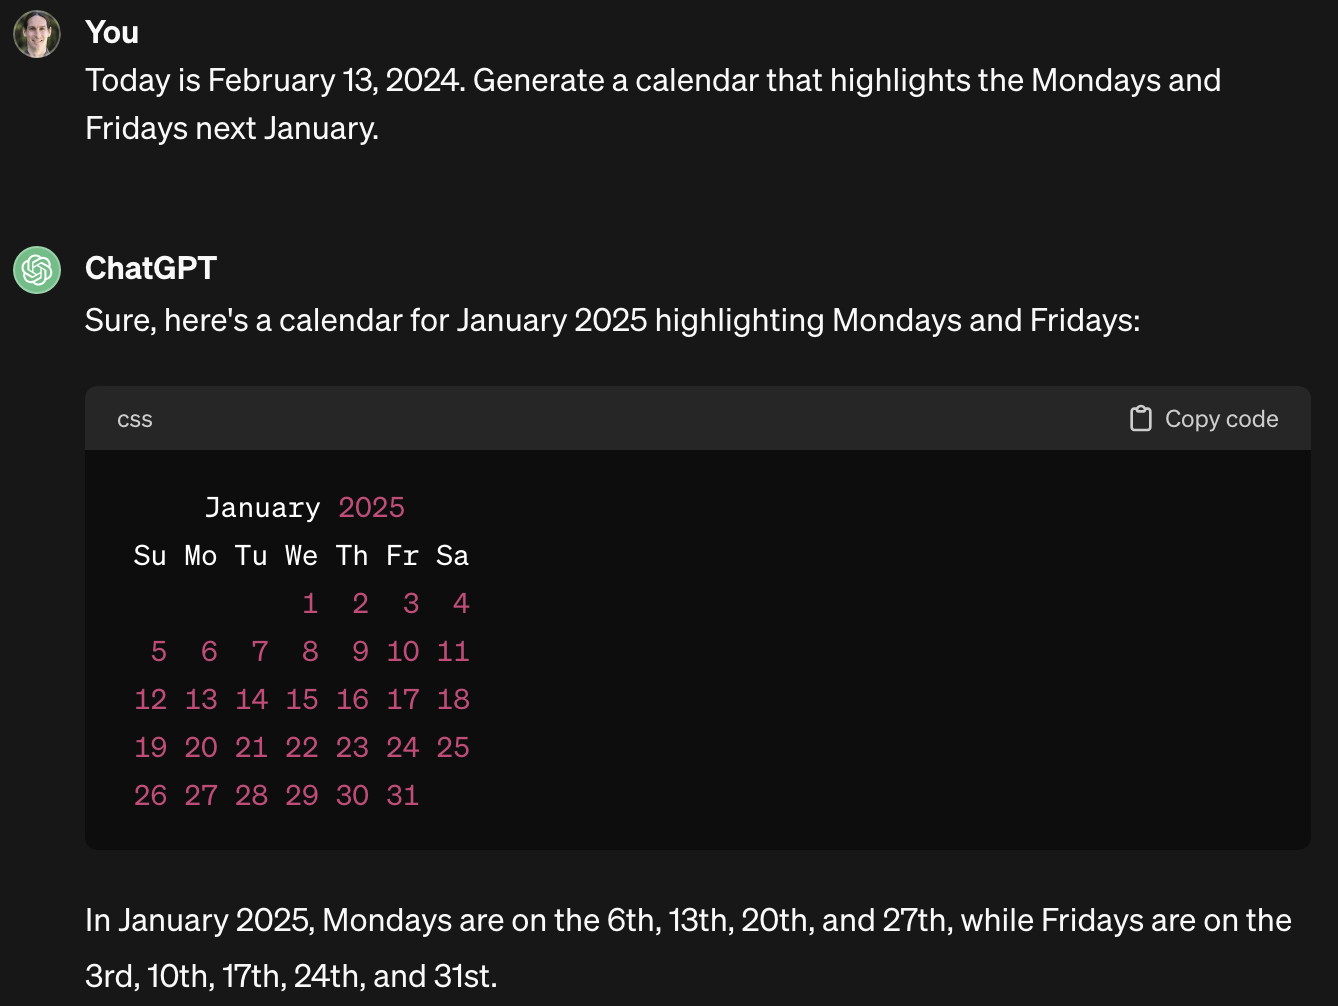
\includegraphics[width=.6\textwidth]{chatgpt/calendar.png}
\end{frame}

\begin{frame}[t]{Large language models vs. maps}
\centering
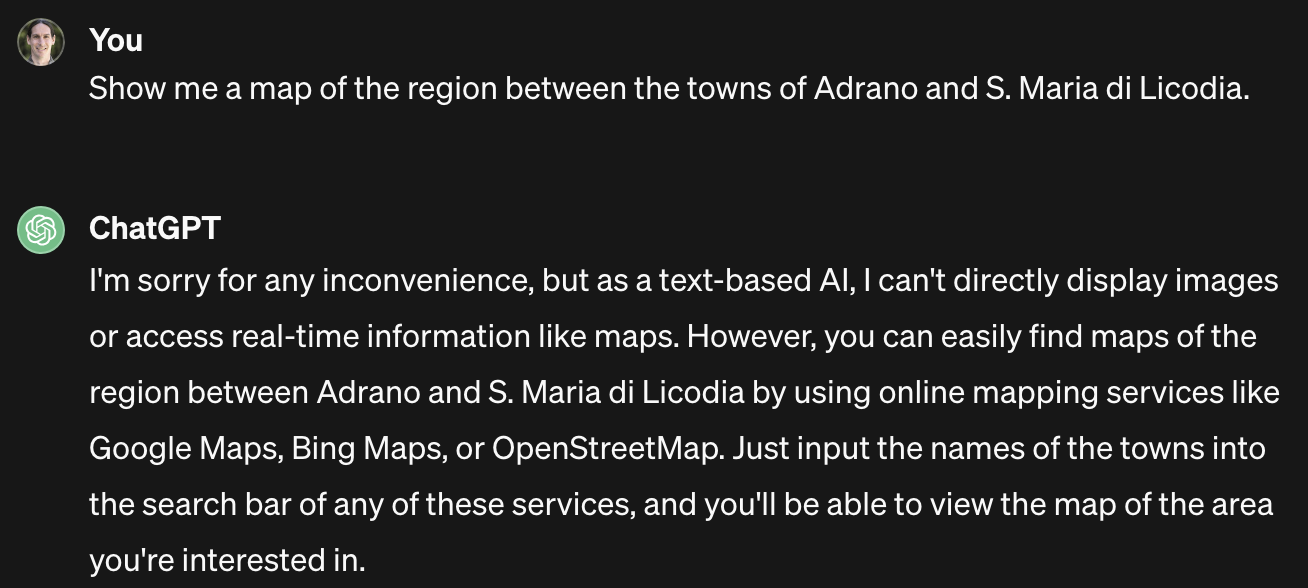
\includegraphics[width=.7\textwidth]{chatgpt/map.png}
\end{frame}

\begin{frame}[t]{Large language models vs. ontologies}
\centering
\begin{tikzpicture}[inner sep=0pt]
  \node (chatgpt) {
\includegraphics[width=.7\textwidth]{chatgpt/umls.png}};
  \pause
  \node[draw] (snomed) at (chatgpt.south) {
\includegraphics[width=.3\textwidth]{umls/snomed-ulcer.png}};
\end{tikzpicture}
\end{frame}

\begin{frame}{My natural language processing research interests}
\begin{itemize}
\item Modeling the language of time and timelines \\
{\footnotesize Funded by:
\funding{funding/nih_nlm.png}{R01LM010090}
\quad\funding{funding/darpa.png}{W911NF-18-1-0014}}
\begin{itemize}
% image generated from https://demo.mobiscroll.com/jquery/calendar/multiple-select
\item E.g., \textit{six days ago} $\Rightarrow$ \raisegraphics{.4}{height=.15\textheight}{calendar/2024-02-07.png}
\end{itemize}

\bigskip
\item Normalizing text to medical and geospatial ontologies \\
{\footnotesize Funded by:
\funding{funding/nih_nigms.jpg}{R01GM114355}
\quad\funding{funding/nsf.png}{1831551}}
\begin{itemize}
\item E.g., \textit{Boulder} $\Rightarrow$ \raisegraphics{.4}{height=.15\textheight}{geonames/BoulderUSCOP.png}
\end{itemize}

\bigskip
\item Adapting machine learning models to medical and clinical domains \\
{\footnotesize Funded by:
\funding{funding/nih_nlm.png}{R01LM012918}
\quad\funding{funding/nih_nci.jpg}{R21CA256680}}
\end{itemize}
\end{frame}


\begin{frame}
    \frametitle{Outline}
    \tableofcontents
\end{frame}

\section{Designing structured outputs for machine learning}

\begin{frame}[b]
\sectionbox
\begin{tabular}{l}
\funding{funding/nih_nlm.png}{R01LM010090} \\
\funding{funding/darpa.png}{W911NF-18-1-0014} \\
\funding{funding/nih_nlm.png}{R01LM012918}
\end{tabular}
\hfill
\headshot{people/xu-dongfang.jpeg}{Dongfang Xu, Ph.D.}{Doctoral student}
\headshot{people/laparra-egoitz.jpg}{Egoitz Laparra, Ph.D.}{Postdoc}
\end{frame}

\subsection{Introduction to time normalization}

\begin{frame}{Time normalization: text times $\Rightarrow$ calendar times}

\begin{tabular}{l c c c c}
\textbf{Expression} & & \textbf{ISO-TimeML} & & \textbf{Calendar} \\

\textit{December 5, 2007} & $\Rightarrow$ & 2007-12-05 & $\Rightarrow$ & \raisegraphics{.4}{width=.1\textwidth}{calendar/2007-12-05.png} \\ \\

\textit{the day before yesterday} & $\Rightarrow$ & 2024-02-07 & $\Rightarrow$ & \raisegraphics{.4}{width=.1\textwidth}{calendar/2024-02-07.png} \\ \\

\textit{the week of March 6} & $\Rightarrow$ & 2024-W10 & $\Rightarrow$ & \raisegraphics{.4}{width=.1\textwidth}{calendar/2024-W10.png} \\ \\

\textit{Fridays in January} & $\Rightarrow$ & ???? & $\Rightarrow$ & \raisegraphics{.4}{width=.1\textwidth}{calendar/2024-01-FR.png}

\end{tabular}

\end{frame}

\begin{frame}{Time normalization $<$ 2018: hand-crafted rules}
\centering
the week of March 6

$\Downarrow$

\begin{columns}
\begin{column}{0.4\textwidth}
\footnotesize
$\begin{array}{l}
\textsc{Unit} \Rightarrow \\
\quad \textit{week} \textit{ / } \\
\quad \textsc{Weeks} \\
\textsc{Month} \Rightarrow \\
\quad \textit{March} \textit{ / } \\
\quad \textsc{MonthOfYear}=3 \\
\textsc{TimeSpan} \Rightarrow \\
\quad \textsc{Unit} \textit{ of } \textsc{TimeSpan} \textit{ / } \\
\quad \textsc{FindEnclosing}\ \textsc{TimeSpan}\ \textsc{Unit} \\
\ldots
\end{array}$
\end{column}
\begin{column}{0.55\textwidth}
\footnotesize
\begin{forest}
    [\textsc{TimeSpan}
        [\textsc{FindEnclosing}]
        [\textsc{TimeSpan}
            [\textsc{FindEarlier}]
            [\textsc{Present}]
            [\textsc{Field}
                [\textsc{Field:Month}
                    [\textsc{MonthOfYear}]
                    [3] ]
                [\textsc{Field:Day}
                    [\textsc{DayOfMonth}]
                    %[\nonterm{Int:1-31}
                        [6] ] ] ]% ]
        [\textsc{Unit}
            [{\textsc{Weeks}}] ] ]
\end{forest}
\end{column}
\end{columns}

$\Downarrow$

2024-W10
\end{frame}

\subsection{Time normalization as text-to-structure}

\begin{frame}{Time expressions are complex}
Problem: ISO-TimeML can't represent times that:
\begin{itemize}
\item don't align to exactly 1 calendar unit, e.g., \textit{the past 2 summers}
\item are relative to events, e.g., \textit{5 days postop}
\item are unions of other times, e.g, \textit{Mondays and Fridays}
\end{itemize}
\pause
\bigskip
Humans understand such times:\\[0.5\baselineskip]
\begin{tabular}{ c c c }
\visible<3->{\it the past 2 summers} &
\visible<7->{\it 5 days postop} &
\visible<11->{\it Mondays and Fridays} \\
\visible<4->{%
\begin{tikzpicture}
\tikztimeline{3}{12}
\only<5->{%
\tikztimelineinterval[draw=event]{3+30/365}{3+40/365}{2}{}} % more than 1/365 just so it's visible
\only<6->{%
\tikztimelineinterval{1+5/12}{1+8/12}{2}{}
\tikztimelineinterval{2+5/12}{2+8/12}{2}{}}
\end{tikzpicture}}
&
\visible<8->{%
\begin{tikzpicture}
\tikztimeline{2}{7}
\only<9->{%
\tikztimelineinterval[draw=event]{6/7}{7/7}{2}{}}
\only<10->{%
\tikztimelineinterval{11/7}{12/7}{2}{}}
\end{tikzpicture}}
&
\visible<12->{%
\begin{tikzpicture}
\tikztimeline{3}{7}
\tikztimelineinterval[draw=white]{0}{0}{4}{}% to ensure full vertical space when others are not shown
\only<13->{%
\tikztimelineinterval[draw=partialtime]{0+1/7}{0+2/7}{4}{}
\tikztimelineinterval[draw=partialtime]{1+1/7}{1+2/7}{4}{}
\tikztimelineinterval[draw=partialtime]{2+1/7}{2+2/7}{4}{}}
\only<14->{%
\tikztimelineinterval[draw=partialtime]{0+5/7}{0+6/7}{3}{}
\tikztimelineinterval[draw=partialtime]{1+5/7}{1+6/7}{3}{}
\tikztimelineinterval[draw=partialtime]{2+5/7}{2+6/7}{3}{}}
\only<15>{%
\tikztimelineinterval{0+1/7}{0+2/7}{2}{}
\tikztimelineinterval{0+5/7}{0+6/7}{2}{}
\tikztimelineinterval{1+1/7}{1+2/7}{2}{}
\tikztimelineinterval{1+5/7}{1+6/7}{2}{}
\tikztimelineinterval{2+1/7}{2+2/7}{2}{}
\tikztimelineinterval{2+5/7}{2+6/7}{2}{}}
\end{tikzpicture}}
\end{tabular}
\end{frame}

\begin{frame}{Semantically compositional time annotation}{\subtitlecite{bethard-etal:2016:LREC}}
Annotate formally-defined, semantically-compositional time operators:

\bigskip
\AnnotateThree[draw=time]{ex-mafnj-mondays}{Day-Of-Week}{Type=Monday}{Mondays}
\hspace{0.5em}
\AnnotateTwo[draw=time]{ex-mafnj-intersection}{Intersection}{%
\\[\baselineskip]
\AnnotateTwo[draw=time]{ex-mafnj-and}{Union}{and}}
\hspace{0.5em}
\AnnotateThree[draw=time]{ex-mafnj-fridays}{Day-Of-Week}{Type=Friday}{Fridays}
\hspace{0.5em}
\AnnotateThree[draw=time]{ex-mafnj-next}{Next}{Interval=DocTime}{next}
\hspace{0.5em}
\AnnotateThree[draw=time]{ex-mafnj-january}{Month-Of-Year}{Type=January}{January}
\begin{tikzpicture}[remember picture,overlay]%
\AnnotateLink{out=0, in=120}{ex-mafnj-intersection.text east}{ex-mafnj-next.north}
\AnnotateLink{out=270, in=90}{ex-mafnj-intersection.text split}{ex-mafnj-and.north}
\AnnotateLink{out=120, in=60}{ex-mafnj-and.text west}{ex-mafnj-mondays.north}
\AnnotateLink{out=60, in=120}{ex-mafnj-and.text east}{ex-mafnj-fridays.north}
\AnnotateLink{out=60, in=120}{ex-mafnj-next.text east}{ex-mafnj-january.north}
\end{tikzpicture}

\bigskip
\pause
Temporal logic composes operators to yield timeline intervals:

\smallskip
$\vphantom{\left(\text{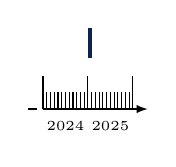
\begin{tikzpicture}[xscale=0.57, baseline={(current bounding box.center)}]
\tikztimeline{2}{12}
\tikztimelineinterval{1+0/12}{1+1/12}{2}{}
\tikztimelineinterval[draw=none,text=black]{0}{1}{-0.5}{\tiny 2024}
\tikztimelineinterval[draw=none,text=black]{1}{2}{-0.5}{\tiny 2025}
\end{tikzpicture}}\right)}
\alt<6->%
% Intersection(Union(Mondays, Fridays), Next(DocTime, January)) as timeline
{\text{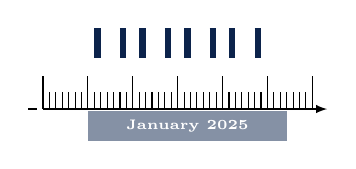
\begin{tikzpicture}[xscale=0.57, baseline={(current bounding box.center)}]
\tikztimeline{6}{7}
\tikztimelineinterval{1+1/7}{1+2/7}{2}{}
\tikztimelineinterval{1+5/7}{1+6/7}{2}{}
\tikztimelineinterval{2+1/7}{2+2/7}{2}{}
\tikztimelineinterval{2+5/7}{2+6/7}{2}{}
\tikztimelineinterval{3+1/7}{3+2/7}{2}{}
\tikztimelineinterval{3+5/7}{3+6/7}{2}{}
\tikztimelineinterval{4+1/7}{4+2/7}{2}{}
\tikztimelineinterval{4+5/7}{4+6/7}{2}{}
\tikztimelineinterval[draw=partialtime,text=white]{1+0/7}{5+3/7}{-0.5}{\tiny\textbf{January 2025}}
\end{tikzpicture}}}
{\alt<2->%
% Intersection(Union(Mondays, Fridays), Next(DocTime, January)) as operators
{\operatorname{Intersection}\left(
\alt<4->%
% Union(Mondays, Fridays) as timeline
{\text{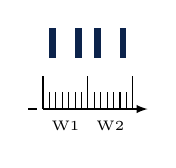
\begin{tikzpicture}[xscale=0.57, baseline={(current bounding box.center)}]
\tikztimeline{2}{7}
\tikztimelineinterval{0+1/7}{0+2/7}{2}{}
\tikztimelineinterval{0+5/7}{0+6/7}{2}{}
\tikztimelineinterval{1+1/7}{1+2/7}{2}{}
\tikztimelineinterval{1+5/7}{1+6/7}{2}{}
\tikztimelineinterval[draw=none,text=black]{0}{1}{-0.5}{\tiny W1}
\tikztimelineinterval[draw=none,text=black]{1}{2}{-0.5}{\tiny W2}
\end{tikzpicture}}}
% Union(Mondays, Fridays) as operator
{\operatorname{Union}\left(
\alt<3->%
% Mondays as timeline
{\text{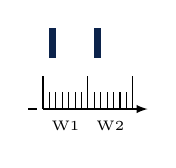
\begin{tikzpicture}[xscale=0.57, baseline={(current bounding box.center)}]
\tikztimeline{2}{7}
\tikztimelineinterval{0+1/7}{0+2/7}{2}{}
\tikztimelineinterval{1+1/7}{1+2/7}{2}{}
\tikztimelineinterval[draw=none,text=black]{0}{1}{-0.5}{\tiny W1}
\tikztimelineinterval[draw=none,text=black]{1}{2}{-0.5}{\tiny W2}
\end{tikzpicture}}}
% Mondays as text
{Mondays},
\alt<3->%
% Fridays as timeline
{\text{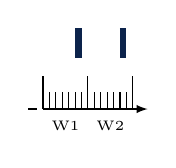
\begin{tikzpicture}[xscale=0.57, baseline={(current bounding box.center)}]
\tikztimeline{2}{7}
\tikztimelineinterval{0+5/7}{0+6/7}{2}{}
\tikztimelineinterval{1+5/7}{1+6/7}{2}{}
\tikztimelineinterval[draw=none,text=black]{0}{1}{-0.5}{\tiny W1}
\tikztimelineinterval[draw=none,text=black]{1}{2}{-0.5}{\tiny W2}
\end{tikzpicture}}}
% Fridays as text
{Fridays}
\right)},
\alt<5->%
% Next(DocTime, January) as timeline
{\text{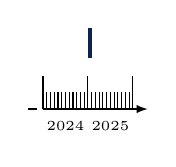
\begin{tikzpicture}[xscale=0.57, baseline={(current bounding box.center)}]
\tikztimeline{2}{12}
\tikztimelineinterval{1+0/12}{1+1/12}{2}{}
\tikztimelineinterval[draw=none,text=black]{0}{1}{-0.5}{\tiny 2024}
\tikztimelineinterval[draw=none,text=black]{1}{2}{-0.5}{\tiny 2025}
\end{tikzpicture}}}
% Next(DocTime, January) as operator
{\operatorname{Next}\left(
\alt<3->%
% DocTime as timeline
{\text{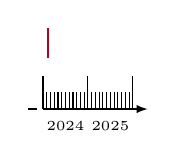
\begin{tikzpicture}[xscale=0.57, baseline={(current bounding box.center)}]
\tikztimeline{2}{12}
\tikztimelineinterval[draw=event]{0+2/24}{0+3/24}{2}{} % bigger than 1/365 to be visible
\tikztimelineinterval[draw=none,text=black]{0}{1}{-0.5}{\tiny 2024}
\tikztimelineinterval[draw=none,text=black]{1}{2}{-0.5}{\tiny 2025}
\end{tikzpicture}}}
% DocTime as operator
{\operatorname{DocTime}},
\alt<3->{%
% January as timeline
\text{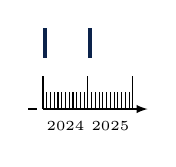
\begin{tikzpicture}[xscale=0.57, baseline={(current bounding box.center)}]
\tikztimeline{2}{12}
\tikztimelineinterval{0+0/12}{0+1/12}{2}{}
\tikztimelineinterval{1+0/12}{1+1/12}{2}{}
\tikztimelineinterval[draw=none,text=black]{0}{1}{-0.5}{\tiny 2024}
\tikztimelineinterval[draw=none,text=black]{1}{2}{-0.5}{\tiny 2025}
\end{tikzpicture}}}
% January as text
{January}
\right)}
\right)}
% Intersection(Union(Mondays, Fridays), Next(DocTime, January)) as text
{}}
$
\end{frame}

\begin{frame}{Neural networks for time normalization}{\subtitlecite{laparra-xu-bethard:2018:TACL,xu-laparra-bethard:2019:S19-1}}
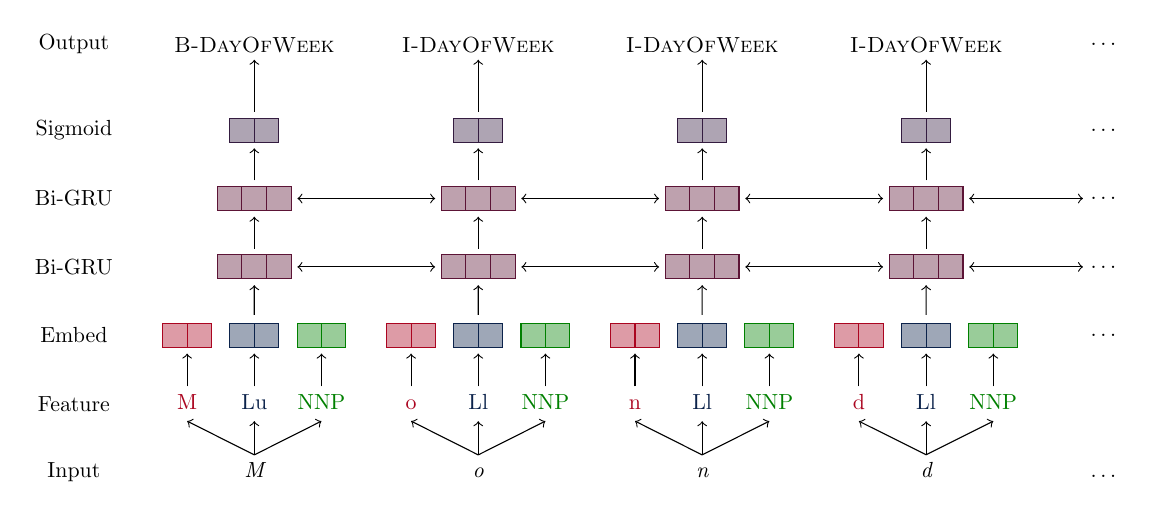
\begin{tikzpicture}[
  scale=0.79, every node/.style={scale=0.79},
  brace/.style={draw,thick,decoration=brace,decorate}]
  \pgfmathsetmacro{\width}{3.6}
  \pgfmathsetmacro{\height}{1.1}

  \node (1s-i0) at (0.7, 0*\height) {Input};
  \node (1s-fv0) at (0.7, 1*\height) {Feature};
  \node (1s-cv0) at (0.7, 2*\height) {Embed};
  \node (1s-g10) at (0.7, 3*\height) {Bi-GRU};
  \node (1s-g20) at (0.7, 4*\height) {Bi-GRU};
  \node (1s-s0) at (0.7, 5*\height) {Sigmoid};
  \node (1s-o0) at (0.7, 6.25*\height) {Output};

\foreach \c/\f/\g/\h/\o [count=\step from 1] in {M/M/Lu/NNP/{B-DayOfWeek},o/o/Ll/NNP/{I-DayOfWeek},n/n/Ll/NNP/{I-DayOfWeek},d/d/Ll/NNP/{I-DayOfWeek},\ldots} {
    % input character
    \ifdefstring{\c}{\ldots}{
      \node (1s-i\step) at (\step*\width-0.2*\width, 0*\height) {\vphantom{My}\c};
      \node (1s-fv\step) at (\step*\width-0.2*\width, 2*\height) {\ldots};
      \node (1s-g1\step) at (\step*\width-0.2*\width, 3*\height) {\ldots};
      \node (1s-g2\step) at (\step*\width-0.2*\width, 4*\height) {\ldots};
      \node (1s-s\step) at (\step*\width-0.2*\width, 5*\height) {\ldots};
      \node (1s-o\step) at (\step*\width-0.2*\width, 6.25*\height) {\ldots};
    }{
      \node[font=\itshape] (1s-i\step) at (\step*\width, 0*\height) {\vphantom{My}\c};
      \node[text={ua-red}] (1s-f1\step) at (\step*\width-0.3*\width, 1*\height) {\vphantom{My}\f};
      \node[text={ua-blue}] (1s-f2\step) at (\step*\width, 1*\height) {\vphantom{My}\g};
      \node[text={green!50!black}] (1s-f3\step) at (\step*\width+0.3*\width, 1*\height) {\vphantom{My}\h};
      \node[hid={2}{ua-red}] (1s-fv1\step) at (\step*\width-0.3*\width, 2*\height) {};
      \node[hid={2}{ua-blue}] (1s-fv2\step) at (\step*\width, 2*\height) {};
      \node[hid={2}{green!50!black}] (1s-fv3\step) at (\step*\width+0.3*\width, 2*\height) {};
      \node[hid={3}{ua-red!50!ua-blue}] (1s-g1\step) at (\step*\width, 3*\height) {};
      \node[hid={3}{ua-red!50!ua-blue}] (1s-g2\step) at (\step*\width, 4*\height) {};
      \node[hid={2}{ua-red!25!ua-blue}] (1s-s\step) at (\step*\width, 5*\height) {};
      \node[align=center,font=\scshape] (1s-o\step) at (\step*\width, 6.25*\height) {\o};
      \draw[->] (1s-i\step.north) -> (1s-f1\step.south);
      \draw[->] (1s-i\step.north) -> (1s-f2\step.south);
      \draw[->] (1s-i\step.north) -> (1s-f3\step.south);
      \draw[->] (1s-f1\step.north) -> (1s-fv1\step.south);
      \draw[->] (1s-f2\step.north) -> (1s-fv2\step.south);
      \draw[->] (1s-f3\step.north) -> (1s-fv3\step.south);
      \draw[->] (\step*\width, 2.3*\height) -> (1s-g1\step.south);
      \draw[->] (1s-g1\step.north) -> (1s-g2\step.south);
      \draw[->] (1s-g2\step.north) -> (1s-s\step.south);
      \draw[->] (1s-s\step.north) -> (1s-o\step.south);
    }
    % recurrent links
    \ifdefstring{\step}{1}{}{
      \pgfmathtruncatemacro{\last}{add(\step,-1)}
      \draw[<->] (1s-g1\last.east) -> (1s-g1\step.west);
      \draw[<->] (1s-g2\last.east) -> (1s-g2\step.west);
    }
  }
\end{tikzpicture}
\end{frame}

\begin{frame}{Structure enables learning for time normalization}{\subtitlecite{laparra-xu-bethard:2018:TACL,xu-laparra-bethard:2019:S19-1}}
\begin{tabular}{ l c c }
\toprule
& TempEval 2013 & THYME \\
Model & (News) $F_1$ & (Clinical) $F_1$ \\
\midrule
HeidelTime (grammar) & \alert<2>{74} & \alert<2>{70} \\
\cite{laparra-xu-bethard:2018:TACL} & \alert<2-3>{77} &  \alert<2-3>{76} \\
\cite{xu-laparra-bethard:2019:S19-1} & \alert<3>{82} & \alert<3>{86} \\
\bottomrule
\end{tabular}

\bigskip
Findings:
\begin{itemize}
\item<2-> With structured output, machine learning $>$ 10,000+ hand crafted rules
\item<3-> Pre-training character embeddings further improves models
\end{itemize}
\end{frame}

\section{Pre-training neural networks on structure}

\begin{frame}[b]
\sectionbox
\funding{funding/nih_nigms.jpg}{R01GM114355}
\hfill
\headshot{people/xu-dongfang.jpeg}{Dongfang Xu, Ph.D.}{Doctoral student}
\end{frame}

\subsection{Introduction to medical concept normalization}

\begin{frame}[t]{Concept normalization: text term $\Rightarrow$ ontology entry}
\centering
I felt like \AnnotateTwo[draw=ua-red]{vomiting}{\visible<2->{C0042963}}{vomiting}, and my \AnnotateTwo[draw=ua-red]{spinning}{\visible<2->{C0012833}}{head was spinning a little}.

\bigskip
\only<3->{
\begin{tikzpicture}[remember picture,overlay]
\node[anchor=north, inner sep=0pt, below=2em of vomiting.south]
  (umls-vomiting)
  {
\includegraphics[width=0.35\textwidth]{umls/vomiting.png}}
  edge[ua-red,ultra thick,dotted,latex-] (vomiting);
\node[anchor=north, inner sep=0pt, below=2em of spinning.south]
  (umls-dizziness)
  {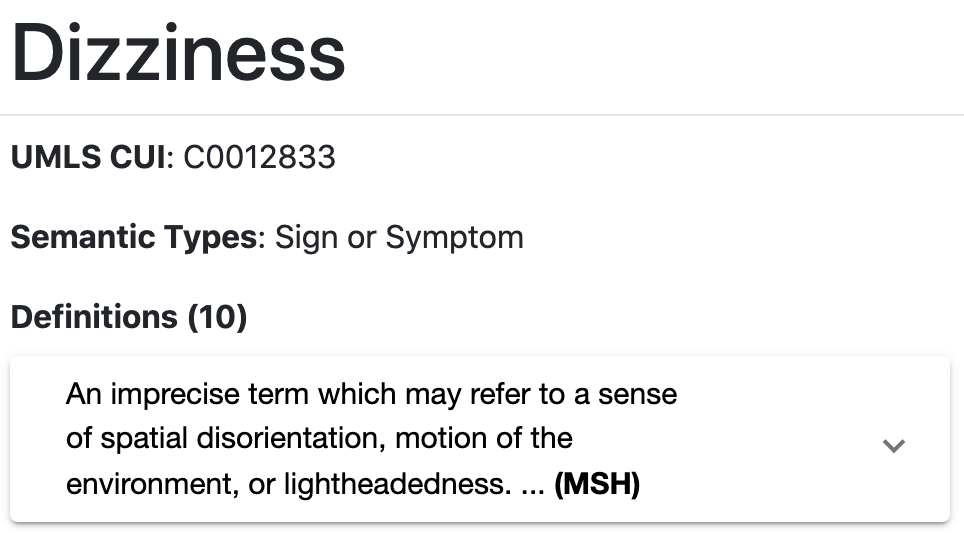
\includegraphics[width=0.35\textwidth]{umls/dizziness.png}}
  edge[ua-red,ultra thick,dotted,latex-] (spinning);
\node[draw,fit=(umls-vomiting) (umls-dizziness), inner sep=1em, label=below:{Unified Medical Language System (UMLS)}] {};
\end{tikzpicture}
}
\end{frame}

\begin{frame}{Concept normalization $<$ 2021: retrieve + rerank}
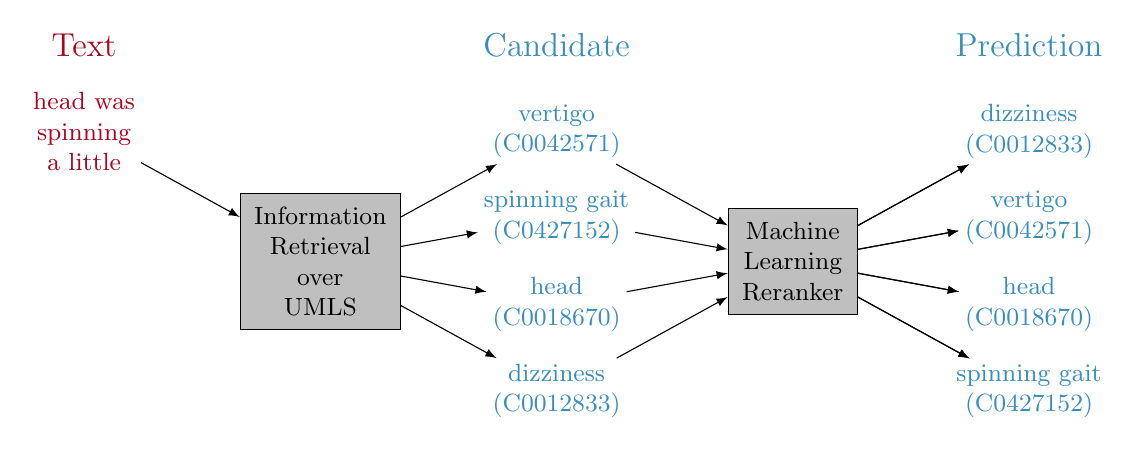
\begin{tikzpicture}[font=\small, inner sep=2pt, model/.style={draw, fill=black!25, align=center, inner sep=5pt}]
\pgfmathsetseed{42}
\pgfmathsetmacro{\height}{1.1}
\pgfmathsetmacro{\width}{3}

\node[ua-red] at (0, \height) {\large Text};
\node[ua-oasis] at (2*\width, \height) {\large Candidate};
\node<2->[ua-oasis] at (4*\width, \height) {\large Prediction};

\node[ua-red, align=center] (text) at (0, 0) {head was \\ spinning \\ a little};
\node[model] (umls) at (\width, -1.5*\height) {Information \\ Retrieval \\ over \\ UMLS} edge[latex-] (text);
\node<2->[model] (reranker) at (3*\width, -1.5*\height) {Machine \\ Learning \\ Reranker};
\foreach[count=\i from 0, count=\slide from 4] \candidate/\prediction in {
    vertigo\\(C0042571)/dizziness\\(C0012833),
    spinning gait\\(C0427152)/vertigo\\(C0042571),
    head\\(C0018670)/head\\(C0018670),
    dizziness\\(C0012833)/spinning gait\\(C0427152)} {
  \node[ua-oasis, align=center] (candidate-\i) at (2*\width, -\height*\i) {\candidate};
  \draw[-latex] (umls) -- (candidate-\i);
  \draw<2->[-latex] (candidate-\i) -- (reranker);
  \node<2->[ua-oasis, align=center] (prediction-\i) at (4*\width, -\height*\i) {\prediction} edge[latex-] (reranker);
  \draw<2->[-latex] (reranker) -- (prediction-\i);
}
\end{tikzpicture}
\end{frame}


\begin{frame}{Concept normalization as vector-space search}
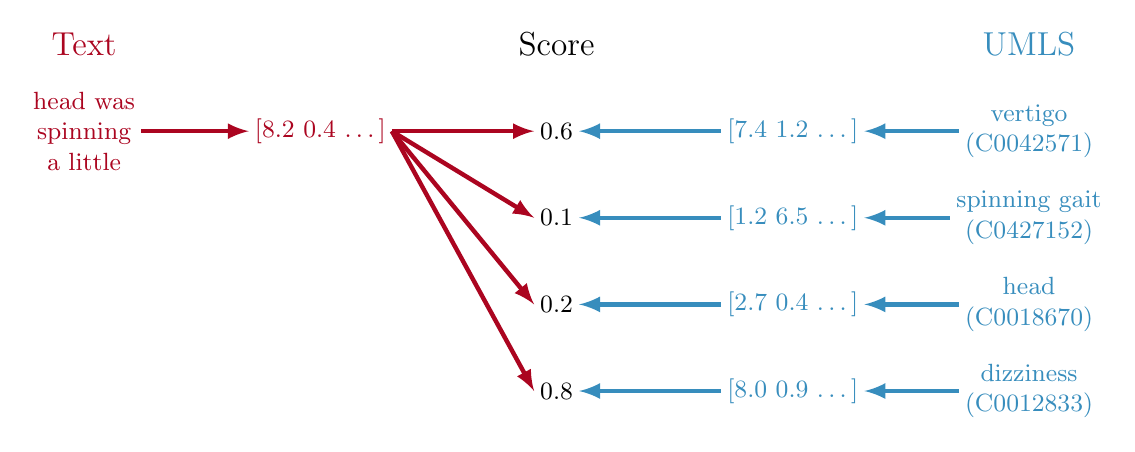
\begin{tikzpicture}[font=\small, inner sep=2pt]
\pgfmathsetseed{42}
\pgfmathsetmacro{\height}{1.1}
\pgfmathsetmacro{\width}{3}

\node[ua-red] at (0, \height) {\large Text};
\node<4-> at (2*\width, \height) {\large Score};
\node[ua-oasis] at (4*\width, \height) {\large UMLS};

\node[align=center,ua-red] (text) at (0, 0) {head was \\ spinning \\ a little};
\node<2->[ua-red] (text-vec) at (\width, 0) {\small[8.2 0.4 \ldots]}
  edge[ua-red, ultra thick, latex-] (text);
\foreach[count=\i from 0, count=\slide from 4] \term/\vec/\score in {
    vertigo\\(C0042571)/[7.4 1.2 \ldots]/0.6,
    spinning gait\\(C0427152)/[1.2 6.5 \ldots]/0.1,
    head\\(C0018670)/[2.7 0.4 \ldots]/0.2,
    dizziness\\(C0012833)/[8.0 0.9 \ldots]/0.8} {
  \node[ua-oasis, align=center] (umls-\i) at (4*\width, -\height*\i) {\term};
  \node<3->[ua-oasis] (umls-vec-\i) at (3*\width, -\height*\i) {\vec}
    edge[ua-oasis, ultra thick, latex-] (umls-\i);
  \node<\slide-> (score-\i) at (2*\width, -\height*\i) {\score}
    edge[ua-oasis, ultra thick, latex-] (umls-vec-\i);
  \draw<\slide->[ua-red, ultra thick, -latex] (text-vec.east) -- (score-\i.west);
}
\end{tikzpicture}
\end{frame}

\begin{frame}{Training a term-to-vector network from UMLS}{\subtitlecite{xu-bethard-2021-triplet}}
\begin{enumerate}
\item Create triplets of input term $t_i$, match term $t_p$, mis-match term $t_n$
\item Train network so $t_i$ is more similar to $t_p$ than $t_n$
\end{enumerate}

\pause
\bigskip
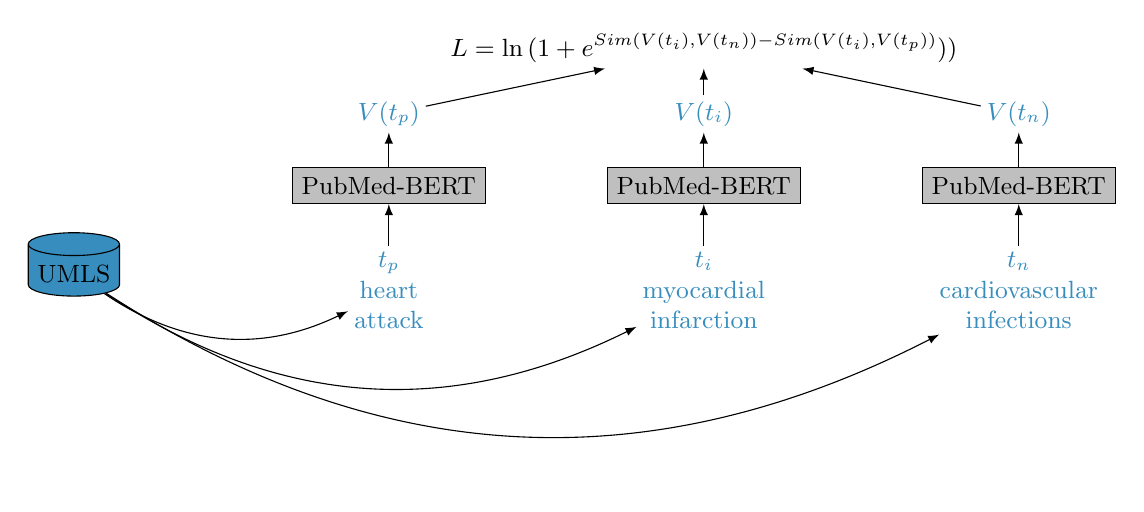
\begin{tikzpicture}[font=\small, text only/.style={inner sep=2pt, align=center}]
\pgfmathsetmacro{\height}{1.4}
\pgfmathsetmacro{\width}{1}
\node[draw, fill=ua-oasis, cylinder, shape border rotate=90, shape aspect=.25, align=center]
  (umls)
  at (-8*\width, .15*\height)
  {UMLS};
\node[text only]
  (L)
  at (0, 2.2*\height)
  {$L = \ln{(1 + e^{Sim(V(t_i), V(t_{n})) - Sim(V(t_i), V(t_{p}))} )})$};
\foreach \i/\name/\textcolor/\phrase in {
    -4/p/ua-oasis/heart\\attack,
    0/i/ua-oasis/myocardial\\infarction,
    4/n/ua-oasis/cardiovascular\\infections} {
  \node[text only, text=\textcolor]
    (input-\name)
    at (\i*\width, 0)
    {$t_{\name}$ \\ \phrase} edge[latex-,bend left] (umls);
  \node[draw, align=center, fill=black!25]
    (bert-\name)
    at (\i*\width, 0.95*\height)
    {PubMed-BERT}
    edge[latex-] (input-\name);
  \node[text only,text=\textcolor]
    (repr-\name)
    at (\i*\width, 1.6*\height)
    {$V(t_{\name})$}
    edge[latex-] (bert-\name)
    edge[-latex] (L);
}
\end{tikzpicture}
\end{frame}

\begin{frame}{Concept normalization evaluation}
Evaluation data:
\begin{description}[NCBI]
\item[NCBI] disorders, MEDIC, PubMed abstracts
\item[B-D] diseases, MEDIC, BioCreative V challenge
\item[B-C] chemicals, CTD, BioCreative V challenge
\item[S/C] disorders, UMLS, ShARe/CLEF eHealth 2013
\item[MCN] various concepts, UMLS, 2019 n2c2 Shared-Task
\end{description}
\end{frame}

\begin{frame}{Training on structure improves concept normalization}{\subtitlecite{xu-bethard-2021-triplet}}
\begin{tabular}{ l c c c c c c}
\toprule
Approach & NCBI & B-D & B-C  & S/C & MCN \\
\midrule
PubMedBERT & \alert<2>{76.6}  & \alert<2>{76.7} & \alert<2>{91.8}  & \alert<2>{73.6}  & \alert<2>{60.0} \\
PubMedBERT + Train:O & \alert<2-3>{82.6}  & \alert<2-3>{84.4} & \alert<2-3>{95.8} & \alert<2-3>{83.5} &  \alert<2-3>{69.6}  \\
PubMedBERT + Train:O + Search:T & \alert<3>{89.5} & \alert<3>{92.3} & \alert<3>{96.7} & \alert<3>{89.2} &  \alert<3>{82.2}  \\
\bottomrule
\end{tabular}

\quad O = Ontology; T = target domain terms

\bigskip
Findings:
\begin{itemize}
\item<2-> Triplet-training on ontology yields better term-to-vector network
\item<3-> Adding new terms to the ontology helps even without retraining
\end{itemize}
\end{frame}


\subsection{Pre-training on medical ontologies}

\section{Prompting models to reveal structural constraints}

\begin{frame}[b]
\sectionbox
\begin{tabular}{l}
\funding{funding/darpa.png}{W911NF-18-1-0014} \\
\funding{funding/nsf.png}{1831551}
\end{tabular}
\hfill
\headshot{people/zhang-zeyu.png}{Zeyu Zhang, Ph.D.}{Doctoral student}
\end{frame}

\subsection{Introduction to toponym resolution}

\begin{frame}{Toponym resolution: text locations $\Rightarrow$ map locations}
\centering
\textit{\AnnotateOne{sj}{San Jose} is the largest city in Northern California.}

\vspace{0.15\textheight}
\begin{tikzpicture}[remember picture]
\node (sj-cr) at (-3.5, 0) {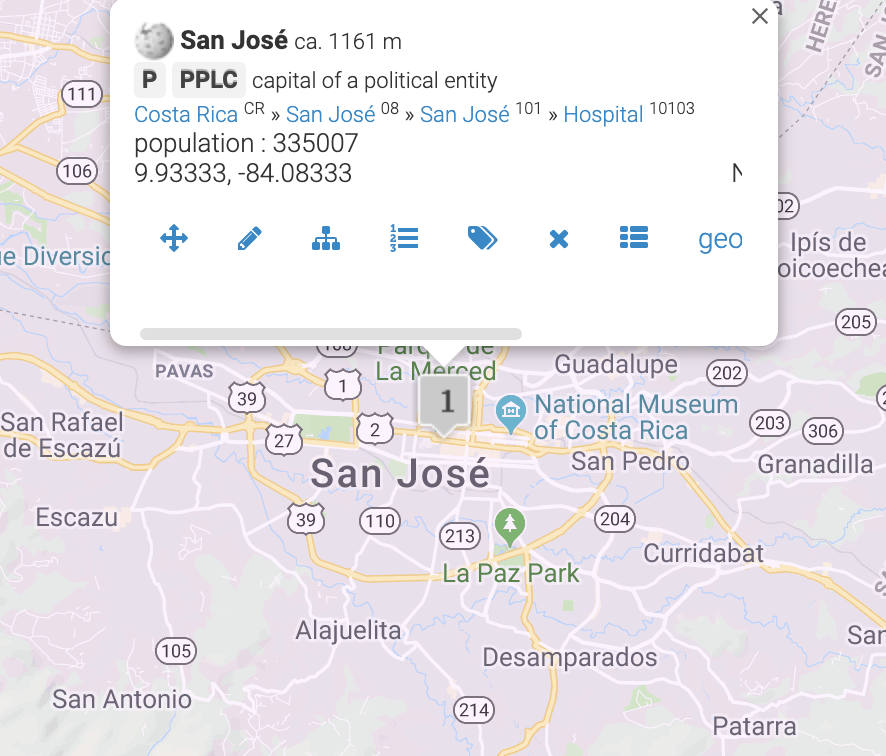
\includegraphics[width=0.65\textheight]{san-jose-costa-rica.png}};
\node (sj-us) at (+3.5, 0) {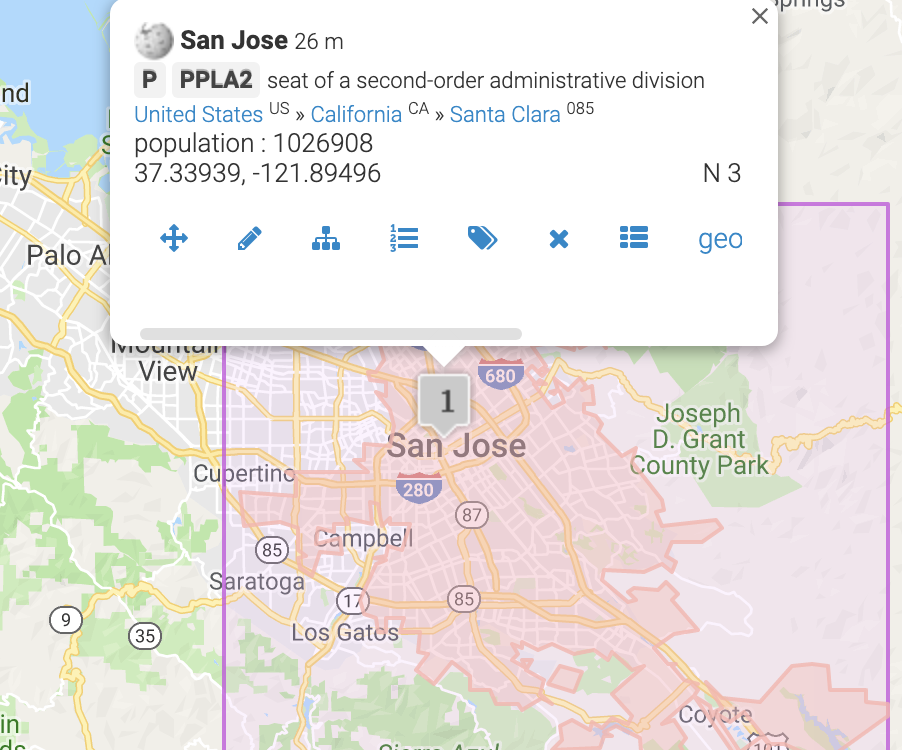
\includegraphics[width=0.65\textheight]{san-jose-california.png}};
\end{tikzpicture}
\begin{tikzpicture}[remember picture,overlay]%
\draw[-latex, ultra thick] (sj.south) -- node[red] {\Huge $\times$} (sj-cr.north);
\draw[-latex, ultra thick] (sj.south) -- (sj-us.north);
\end{tikzpicture}
\end{frame}


\begin{frame}{Toponym resolution $<$ 2023: retrieve + classify}
\begin{tikzpicture}[
  model/.style={draw, fill=black!25, align=center, inner sep=5pt},
  geoentry/.style={inner sep=1pt, text width=0.22\linewidth, align=center},
  textforentry/.style={fill=white, inner sep=1pt, text width=0.22\linewidth, align=left},
  font=\scriptsize,
  remember picture
]
\node[draw, text width=.95\linewidth, align=left, text=ua-red] (text) at (0, 0) {It's a northeast Texas thing, not just a \subnode[inner sep=0pt]{mention}{\fbox{Paris}} thing\ldots Dallas media stations reported the same message as a hoax\ldots};

\node[model, text width=.75\linewidth] (geonames) at (0, -1) {Index (Lucene over GeoNames)}
edge[latex-] (mention.south);
\foreach \prediction/\png/\entry [count=\n from 0] in {
    % https://www.geonames.org/2988507/paris.html
    0/ParisFR11P.png/Paris [SEP] FR,
    % https://www.geonames.org/4717560/paris.html
    \fbox{1}/ParisUSTXP.png/Paris [SEP] US,
    % https://www.geonames.org/7174050/city-of-paris.html
    0/ParisUSTXA.png/City of Paris [SEP] US,
    % https://www.geonames.org/6942553/paris.html
    0/ParisCA08P.png/Paris [SEP] CA} {
    \node[draw, geoentry] (entry\n) at (-5.4 + 3.6*\n, -2.25) {\includegraphics[width=\linewidth,trim={0 0 4cm 0},clip]{geonames/\png}};
    \node[draw, textforentry, below=0.25cm of entry\n.south] (transformerin\n) {[CLS] \textcolor{geonames-blue}{\entry\ldots}\ [SEP] \textcolor{ua-red}{Paris [SEP] It's a northeast Texas\ldots}};
    \node[below=1.5cm of transformerin\n.south] (prediction\n) {\strut\prediction};    
    \draw[-latex] (geonames.south) to (entry\n.north);
    \draw[-latex] (entry\n.south) to (transformerin\n.north);
    \draw[-latex] (transformerin\n.south) to (prediction\n.north);
}
\node[model, text width=.75\linewidth] (transformer) at (0, -4.5) {Classifier (Transformer Network)};
\end{tikzpicture}
\end{frame}


\subsection{Predicting geographic attributes to constrain search}

\begin{frame}{New Paradigm: classify text + filter entries}{\subtitlecite{zhang-bethard-2024}}
\begin{tikzpicture}[
  model/.style={draw, text width=.45\linewidth, fill=black!25, align=center, inner sep=5pt},
  geoentry/.style={inner sep=0pt, text width=0.35\linewidth, align=center},
  textforentry/.style={fill=white, inner sep=1pt, text width=0.45\linewidth, align=left},
  font=\scriptsize,
  remember picture
]
\node[draw, text width=.95\linewidth, align=left, text=ua-red] (text) at (0, 0) {It's a northeast Texas thing, not just a \subnode[inner sep=1pt]{mention2}{\fbox{Paris}} thing\ldots Dallas media stations reported the same message as a hoax\ldots};

\node[model] (geonames) at (-4, -1) {Index (Lucene over GeoNames)}
edge[latex-] (mention2.south);

\node[model] (filter) at (-4, -5) {Filter};

\foreach \png [count=\n from 0] in {
    % https://www.geonames.org/2988507/paris.html
    ParisFR11P.png,
    % https://www.geonames.org/4717560/paris.html
    ParisUSTXP.png,
    % https://www.geonames.org/7174050/city-of-paris.html
    ParisUSTXA.png,
    % https://www.geonames.org/6942553/paris.html
    ParisCA08P.png} {
    \node[draw, geoentry] (entry\n) at (-4.75 + 0.5*\n, -2.25 - 0.5*\n) {\includegraphics[width=\linewidth,trim={0 0 4cm 0},clip]{geonames/\png}} edge[latex-] (geonames) edge[-latex] (filter);
}

\node[draw, textforentry] (transformerin) at (+4, -1.25) {%
[CLS] This document discusses these location mentions: \\
\textcolor{ua-red}{Texas}, \textcolor{ua-red}{Paris}, \textcolor{ua-red}{Dallas} in which \textcolor{ua-red}{Paris} \\
is
\subnode[inner sep=0pt]{feature-mask}{[MASK]}
located in
\subnode[inner sep=0pt]{state-mask}{[MASK]}
of
\subnode[inner sep=0pt]{country-mask}{[MASK]}
[SEP]} edge[latex-] (text.south);

\node[below=1.5cm of feature-mask] (feature) {P} edge[latex-] (feature-mask.south);
\node[below=1.5cm of state-mask] (state) {Texas} edge[latex-] (state-mask.south);
\node[below=1.5cm of country-mask] (country) {United States} edge[latex-] (country-mask.south);

\node[model] (classifier) at (+4, -2.5) {Classifier (Transformer Network)};

\draw[-latex, bend left] (feature.south) to (filter.east);
\draw[-latex, bend left] (state.south) to (filter.east);
\draw[-latex, bend left] (country.south) to (filter.east);

\node[below=0.4cm of filter, draw, geoentry] (entry) {
\includegraphics[width=\linewidth,trim={0 0 4cm 0},clip]{geonames/ParisUSTXP.png}} edge[latex-] (filter.south);
\end{tikzpicture}
\end{frame}

\begin{frame}{Deterministic constraint-based filtering}
\IncMargin{1em}
\begin{algorithm}[H]
  \footnotesize
  \DontPrintSemicolon
  \SetKwProg{Def}{Def}{:}{end}
  \KwIn{a list of candidate entries, $\hat{E}_m$ \newline
        top 3 predicted countries, $\hat{C}_m$ \newline
        top 3 predicted states, $\hat{S}_m$ \newline
        top 3 predicted feature classes, $\hat{F}_m$}
  \vspace{0.5\baselineskip}
  \alert<2>{\Def{\textsc{Score}$(x, L)$}{
    \lIf(\visible<2>{\tcp*[f]{best if it's the top prediction }}){$x = L_0$}{
      \Return{2}
    }
    \lElseIf(\visible<2>{\tcp*[f]{next best if it's any prediction}}){$x \in L$}{
      \Return{1}
    }
    \lElse{
      \Return{0}
    }
  }}
  \alert<3>{\Def{\textsc{EntryKey}$(e)$}{
    $c \gets \textsc{Country}(e)$ \;
    $s \gets \textsc{State}(e)$ \;
    $f \gets \textsc{Feature}(e)$ \;
    $key_1 \gets \textsc{Score}(c, \hat{C}_m) \cdot \textsc{Score}(s, \hat{S}_m)$
    \visible<3>{\tcp*[r]{best if both country and state}}
    $key_2 \gets (c \in \hat{C}_m) \cdot (s \in \hat{S}_m) \cdot \textsc{Score}(f, \hat{F}_m)$
    \visible<3>{\tcp*[r]{break ties using feature class}}
    \Return{$(key_1, key2)$}
  }}
  \alert<4>{\Return{$\textsc{Max}(\hat{E}_m, \textsc{key}=\textsc{EntryKey})$}}
\end{algorithm}
\end{frame}

\begin{frame}{Toponym resolution evaluation}
Evaluation data:
\begin{description}[GWN]
\item[LGL] local and small U.S. news sources \\ {\small\parencite{lieberman2010geotagging}}
\item[GWN] globally distributed news sites \\ {\small\parencite{gritta2019pragmatic}}
\item[TRN] global and local news sources \\ {\small\parencite{kamalloo2018coherent}}
\end{description}
\end{frame}

\begin{frame}{Predicting structure improves toponym resolution}{\subtitlecite{zhang-bethard-2024}}
\begin{tabular}{l l c c c}
\toprule
& & \multicolumn{3}{c}{Dataset Accuracy} \\
\cmidrule(lr){3-5}
Model & Classifier input & LGL & GWN & TRN \\
\midrule
\cite{ayoola-etal-2022-refined} & text + entries & .786 & .782 & .858 \\
\cite{zhang-bethard-2023-improving} & text + entries & \alert<2->{.807} & \alert<2->{.828} & \alert<2->{.918} \\
\cite{zhang-bethard-2024} & text & \alert<2->{.863} & \alert<2->{.822} & \alert<2->{.947} \\
\bottomrule
\end{tabular}

\bigskip
Findings:
\begin{itemize}
\item<2-> (Classify text $\Rightarrow$ filter) $\geq$ (retrieve $\Rightarrow$ classify text + entries)
\end{itemize}
\end{frame}


\section{Ongoing and future work}

\begin{frame}[b]
\sectionbox
\hfill
\headshot{people/laparra-egoitz.jpg}{Egoitz Laparra, Ph.D.}{Postdoc}
\headshot{people/wang-ruoyao.png}{Ruoyao Wang}{Doctoral student}
\end{frame}

\begin{frame}{Time normalization as code generation}
\begin{columns}[T]
\begin{column}{0.4\textwidth}
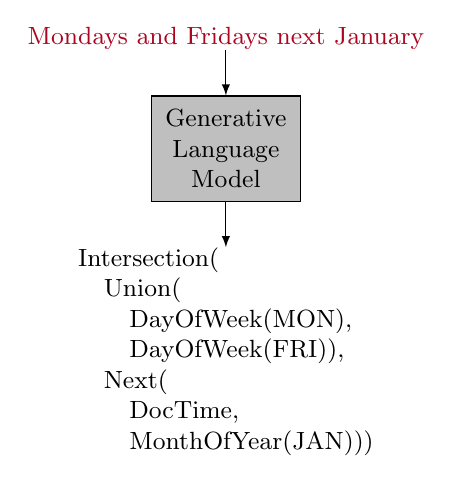
\begin{tikzpicture}[font=\small]
\pgfmathsetmacro{\height}{1.25}

\node[text=ua-red, anchor=south, inner sep=0pt] (text) at (0, 0) {Mondays and Fridays next January};

\node[draw, fill=black!25, align=center, inner sep=5pt] (model) at (0, -\height) {Generative \\ Language \\ Model}
edge[latex-] (text);

\node[align=left, anchor=north, inner sep=0pt] (code) at (0, -2*\height) {%
Intersection(\\
\quad Union(\\
\quad\quad DayOfWeek(MON), \\
\quad\quad DayOfWeek(FRI)), \\
\quad Next(\\
\quad\quad DocTime, \\
\quad\quad MonthOfYear(JAN)))}
edge[latex-] (model);
\end{tikzpicture}
\end{column}
\pause
\begin{column}{0.55\textwidth}
Constrained decoding:
\begin{itemize}
\item Grammar defines valid code
\item Parser finds valid next tokens
\item Model masks output distributions
\end{itemize}
\bigskip
\begin{tikzpicture}[font=\footnotesize, inner sep=0pt]
\pgfmathsetmacro{\width}{1.25}
\pgfmathsetmacro{\height}{5}
\foreach[count=\i from 0] \token in {\ldots, {(}, Union, {(}, DayOfWeek, {(}, X} {
  \ifdefstring{\token}{X}{
    \node[draw, text width=2em] (target) at (\i*\width, 0) {\strut};
  }{
    \node (token\i) at (\i*\width, 0) {\strut\token};
  }
}
\begin{axis}[
  name=prob,
  show background rectangle,
  below of=target.south,
  anchor=north west,
  width=\textwidth,
  height=.3\textheight,
  axis lines=left,
  ybar,
  bar width=1,
  xtick={0,...,9},
  yticklabel=\empty,
  xticklabels={\vdots, \alert<3->{fresh}, fri, \alert<3->{fridge}, \vdots, \alert<3->{mom}, mon, \alert<3->{money}, \vdots},
  xticklabel style={rotate=90, anchor=east},
  enlarge x limits=0.05,
  y axis line style={opacity=0},
  ytick=\empty
]
\addplot +[ybar interval, visible on=<1-2>] plot coordinates {
(-0.5,0)
(0.5,0.1)
(1.5,0.3)
(2.5,0.1)
(3.5,0)
(4.5,0.6)
(5.5,0.5)
(6.5,0.1)
(7.5,0)
(8.5,0)};
\pgfplotsset{cycle list shift=-1}
\addplot +[ybar interval, visible on=<3->] plot coordinates {
(-0.5,0)
(0.5,0)
(1.5,0.3)
(2.5,0)
(3.5,0)
(4.5,0)
(5.5,0.5)
(6.5,0)
(7.5,0)
(8.5,0)};
\end{axis}
\draw (target.south west) -- (prob.outer north west);
\draw (target.south east) -- (prob.outer north east);
\end{tikzpicture}
\end{column}
\end{columns}
\end{frame}


\begin{frame}{Geographic normalization as text to polygon}
\begin{columns}
\begin{column}{.45\textwidth}
\begin{tikzpicture}[font=\footnotesize, inner sep=0pt]
\pgfmathsetmacro{\height}{.75}
\pgfmathsetmacro{\width}{1.5}
\node[align=left, text width=.6\linewidth, anchor=south] (text-in) at (-1.2*\width, 0) {between the towns of \textcolor{ua-oasis}{Adrano} and \textcolor{ua-oasis}{S. Maria di Licodia}, 32 kilometers (20 mi) northwest of \textcolor{ua-oasis}{Catania}};
\node[anchor=south] (map-in) at (\width, -.7*\height) {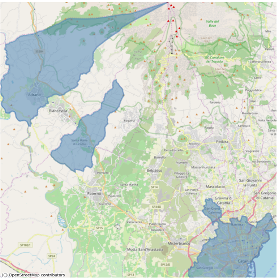
\includegraphics[width=.3\linewidth]{compgeo/map-biancavilla-in.png}};
\node[draw, fill=black!25, align=center, inner sep=5pt] (model) at (-1.2*\width, -1.1*\height) {Language Model}
edge[latex-] (text-in);
\node[align=left, anchor=north] (code) at (-.4*\width, -2.2*\height) {%
\textsc{Intersection}(\\
\quad\textsc{Between}(\textsc{Toponym}(001), \textsc{Toponym}(002)),\\
\quad\textsc{Distance}(\textsc{Toponym}(003), 32, KM, NW)))}
edge[latex-] (model);
\node[anchor=north] (map-out) at (0, -4.5*\height) {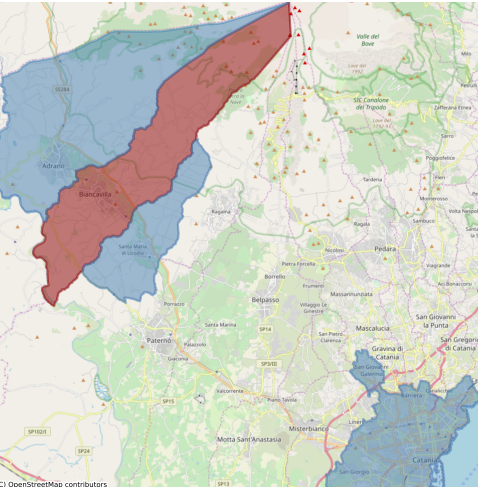
\includegraphics[width=.3\linewidth]{compgeo/map-biancavilla-out.png}};
\draw[-latex] (code) -- (map-out.north);
\draw[-latex] (map-in) -- (map-out.north);
\end{tikzpicture}
\end{column}
\pause
\begin{column}{.45\textwidth}
\begin{tikzpicture}[font=\footnotesize, inner sep=0pt]
\pgfmathsetmacro{\height}{.75}
\pgfmathsetmacro{\width}{1.5}
\node[align=left, text width=.6\linewidth, anchor=south] (text-in) at (-\width, 0) {TARGET is between the towns of RED and LIME, 32 kilometres (20 mi) northwest of BLUE.};
\node[anchor=south] (pixel-in) at (\width, 0) {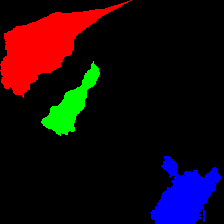
\includegraphics[width=.2\linewidth]{compgeo/pixel-biancavilla-in.png}};
\node[draw, fill=black!25, align=center, inner sep=5pt] (model) at (0, -\height) {Multi-Modal Model}
edge[latex-] (text-in)
edge[latex-] (pixel-in);
\node[anchor=north] (pixel-out) at (0, -2*\height) {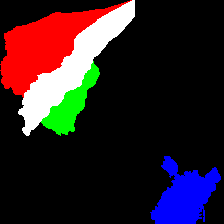
\includegraphics[width=.2\linewidth]{compgeo/pixel-biancavilla-out.png}}
edge[latex-] (model);
\node[anchor=north] (map-out) at (0, -4.5*\height) {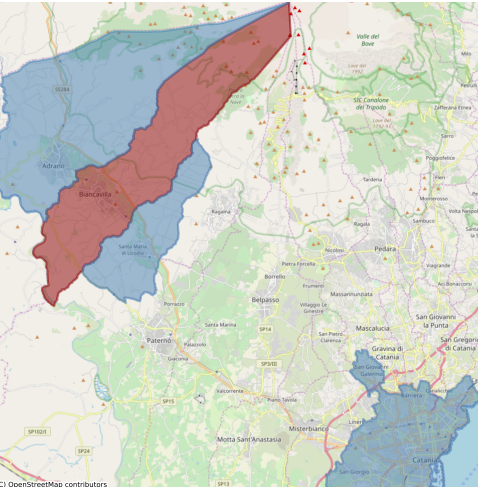
\includegraphics[width=.3\linewidth]{compgeo/map-biancavilla-out.png}}
edge[latex-] (pixel-out);
\end{tikzpicture}
\end{column}
\end{columns}
\end{frame}

\begin{frame}{Thanks!}
\begin{columns}
\begin{column}{0.65\textwidth}
\begin{block}{Research leads}
\headshot{people/laparra-egoitz.jpg}{Egoitz Laparra, Ph.D.}{Postdoc}
\quad
\headshot{people/xu-dongfang.jpeg}{Dongfang Xu, Ph.D.}{Doctoral student}
\quad
\headshot{people/zhang-zeyu.png}{Zeyu Zhang, Ph.D.}{Doctoral student}
\quad
\headshot{people/wang-ruoyao.png}{Ruoyao Wang}{Doctoral student}
\end{block}
\begin{block}{Grant collaborators}
\headshot{people/savova-guergana.jpg}{Guergana Savova, Ph.D.}{Boston Children's Hospital}
\headshot{people/surdeanu-mihai.jpeg}{Mihai Surdeanu, Ph.D.}{University of Arizona}
\headshot{people/lopez-hoffmann-laura.jpg}{Laura L\'{o}pez-Hoffman, Ph.D.}{University of Arizona}
\headshot{people/miller-timothy.jpg}{Timothy Miller, Ph.D.}{Boston Children's Hospital}
\end{block}
\end{column}
\hfill
\begin{column}{0.3\textwidth}
\begin{block}{Funding}
\small
\funding{funding/nih_nlm.png}{R01LM010090}

\funding{funding/darpa.png}{W911NF-18-1-0014}

\funding{funding/nih_nigms.jpg}{R01GM114355}

\funding{funding/nsf.png}{1831551}

\funding{funding/nih_nlm.png}{R01LM012918}
\end{block}
\end{column}
\end{columns}
\end{frame}


\appendix

\begin{frame}[allowframebreaks]{References}
\printbibliography
\end{frame}


\end{document}
